\chapter{Methodology \label{ch:methodology}}
This chapter presents the hard- and software used in the \ac{ADS} as it was prepared for the junior flight of \ac{SETH}, the sensor calibration technique, and the calculation of pitch, roll, and heading. The methodology covers a mixture of work done by senior scientists of the \ac{IEAP} and our contributions. The most notable external contribution comes from Dr. Stephan Böttcher, who did the \ac{PCB} design, wrote the \ac{FPGA} code and soldered the example which was used. 

\begin{figure}[H]
    \centering
    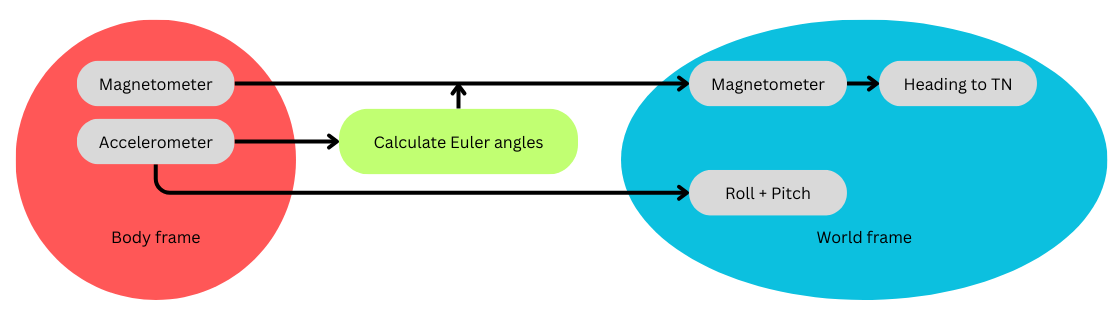
\includegraphics[width=0.75\linewidth]{images/02_methodology/ads_flowchart.png}
    \caption{Flowchart of the methodology.}
    \label{fig:meth:ads_flowchart}
\end{figure}

Figure~\ref{fig:meth:ads_flowchart} shows the processes used to fulfil

\section{Data Acquisition \label{sec:meth:data_acquisition}}
The data produced by the accelerometer and magnetometer is stored in \ac{FIFO} buffers until it is requested by the \ac{FPGA}. Once requested, the program \verb|rpirena.py| is used to stream the data coming from the \ac{FPGA} to the SD\:Card or a file on a server. This program was written by Dr. Stephan Böttcher and runs on a Raspberry Pi Zero. The program writes different event lines into a file, depending on the header of the packet taken from the \ac{FIFO}. The important lines for this thesis are the \verb|ID| lines. These lines contain the information from the accelerometer and magnetometer, each entry separated by a white space. Except for the line identifier, all other values are decimal representations of an unsigned 16-bit number, called a word.

The first entry is the line identifier \say{ID}, followed by the packet header 4805$\equiv$0x12C5. After this, the number of words in the line minus one (the packet header is not counted towards this number) is printed. This number is 132 by design. After this number, the information words from the accelerometer and magnetometer begin. The first word is the magnetometer status register. This contains information if and if so, what data was overwritten, and if new data is available. Words three through five are the data output registers in order~X,~Y, and~Z. Word six is the temperature data from the magnetometer. Words seven, eight, nine, and ten are accelerometer registers containing information about the auxiliary \acp{ADC}. The next batch of words, 11 through 64, are 18 magnetometer vectors, one after the other and each in order~X,~Y, and~Z. Word 65 is the FIFO\_SRC register of the accelerometer with information about the data contained in the \ac{FIFO}. Word 66 is the status register. Words 67 through 126 are 21 accelerometer vectors in the same order as the magnetometer. One more magnetometer vector is read from the last three words, 130, 131 and 132. This is illustrated below:
\begin{lstlisting}
#   0     1    2     3    6     7     11   65    66    67   130
ID  4805  132  STAT  MAG  TEMP  STAT  MAG  FIFO  STAT  ACC  MAG
\end{lstlisting}

Because the \acp{FIFO} are read every two seconds, the last magnetometer and accelerometer vector is the same as the second-to-last.

\section{Data Interpretation \label{sec:meth:data_interpretation}}
Instances of the \textit{ads} class from the \verb|python| script \verb|att_eval.py| are used to interpret the data. Each instance is an object of a specific \verb|.EI| file. The whole file is read with python's built-in \textit{.lineread()} method. The vectors between two housekeeping (\say{H}) lines are written into an array with $n\cdot20$ lines and 6 columns, where $n$ is an integer equal to the number of \say{ID} lines between the two \say{H} lines. The times of the vectors are calculated by setting the time of the first vector as the time in the first \say{H} line minus one second. All the following times are then in $100\,\mathrm{ms}$ steps until the time in the second \say{H} line minus 1 second is reached. The start time must start one second earlier because the time that the vectors are measured and digitalized is two seconds before the time when they are requested by the \ac{FPGA}.

The methods \textit{.plot\_vectors()}, \textit{.plot\_sphere()}, \textit{.plot\_angles()}, and \textit{.plot\_heading()} are used to display the specified data. The methods plot the following data: The components of the accelerometer and magnetometer, converted to $\mathrm{mGs}$ and units of $g$, against time, the components in three-dimensional space, the calculated pitch and roll angles against time, and the calculated pitch and roll angles, as well as the heading, against time.

\section{Sensor Calibration Technique \label{sec:meth:calibration_technique}}
\cite{non-orthonogality} present the technique which is applied to calibrate the magnetometer and accelerometer. The calibration relies only on the magnitude of the vector field to be measured. This is due to the insight that the flawless measurements of the sensors plotted in three-dimensional space all fall onto the surface of a sphere, and the radius of the sphere is simply the magnitude of the vector field to be measured. For the earth's magnetic field, $\vec{B}_H$, this is:
\begin{align}
    \vec{B}_H&=\begin{pmatrix} B_x \\ B_y \\ B_z \end{pmatrix} \label{eq:earth_field} \\
    \iff B_H^2& = B_x^2+B_y^2+B_z^2 
    \label{eq:regular_sphere}
\end{align}

If we assume the measurement of each component of the field to be affected by a scale factor and a linear offset, we get the following three equations. The field to be measured is given as in~\eqref{eq:earth_field}, and we use the superscript~$B$ to denote that these are the coefficients for the measurement of the magnetometer.
\begin{align}
    B_{x,\mathrm{meas}} &= \frac{B_x}{\sqrt{a^B}}+x_0^B \\
    B_{y,\mathrm{meas}} &= \frac{B_y}{\sqrt{b^B}}+y_0^B \\
    B_{z,\mathrm{meas}} &= \frac{B_z}{\sqrt{c^B}}+z_0^B
\end{align}

Solving for $B_{x,y,z}$ in each of the formulae above gives us:
\begin{align}
    B_x&=\sqrt{a^B}(B_{x,\mathrm{meas}}-x_0^B) \label{eq:bx} \\
    B_y&=\sqrt{b^B}(B_{y,\mathrm{meas}}-y_0^B) \label{eq:by} \\
    B_z&=\sqrt{c^B}(B_{z,\mathrm{meas}}-z_0^B) \label{eq:bz}
\end{align}

Plugging eqs.~\eqref{eq:bx} to~\eqref{eq:bz} into eq.~\eqref{eq:regular_sphere} gives us the formula for an ellipsoid shifted off the origin by~$x_0^B$,~$y_0^B$, and~$z_0^B$. The half-axes of the ellipsoid are given by the scale factors.
\begin{equation}
    B_{H}^2=a^B(B_{x,\mathrm{meas}}-x_0^B)^2 + b^B(B_{y,\mathrm{meas}}-y_0^B)^2 + c^B(B_{z,\mathrm{meas}}-z_0^B)^2 
    \label{eq:mag_fit_function}
\end{equation}

 We use equation~\eqref{eq:mag_fit_function} to determine the coefficients $a^B$,~$b^B$,~$c^B$,~$x_0^B$,~$y_0^B$ and~$z_0^B$ with \verb|gnuplot|'s fit function. The measured vectors are given as input for the right-hand side of the equation, while the square of the magnitude of the Earth's magnetic field in Kiel is used for the left hand side.\\
It is now also apparent why we chose the scale factors in eqs.~\eqref{eq:bx}~-~\eqref{eq:bz} as one over the square root: the fit converges faster and more accurately when fitting a linear relationship.

Although we derived eq.~\eqref{eq:mag_fit_function} for the Earth's magnetic field, we apply the same concept in the calibration of the accelerometer. The function used to determine the coefficients is eq.~\eqref{eq:acc_fit_function}. Because the data is in units of~$g$ the magnitude of the field is~1.
\begin{equation}
    1\overset{!}{=}a^g(g_{x,\mathrm{meas}}-x_0^g)^2 + b^g(g_{y,\mathrm{meas}}-y_0^g)^2 + c^g(g_{z,\mathrm{meas}}-z_0^g)^2
    \label{eq:acc_fit_function}
\end{equation}

After determining the coefficients $a$,~$b$,~$c$,~$x_0$,~$y_0$, and~$z_0$ for the accelerometer and magnetometer, the measured data set is modified as given in eqs.~\eqref{eq:bx}~-~\eqref{eq:bz} to get the true components without measurement error.

We perform a calibration measurement to compare two possible calibration methods. The first method is placing the sensor in a given orientation for a time of about 60\,s. A new orientation is chosen very 60\,s after this, placing the sensor on a new face of the housing each time. Once all sides (except for the one with the connector) have faced down once, a second method is tested in the same measurement run. The second method is called a "random tumble" in allusion to a random walk. In this random tumble, the sensor is rotated randomly around its centre point at a height of around 1.7\,m. To verify the best calibration method, the following steps are performed:
\begin{enumerate}
    \item fit coefficients calculated for method I, method II and both
    \item calibrate data set with each set of coefficients
    \item residuals calculated for each set
    \item mean and standard deviation for each residual calculated
    \item the set with the lowest mean residual is chosen as optimal parameters
\end{enumerate}
The residuals~$\Delta B$ of the magnitude of the magnetic field~$B=|\vec{B}|$ are calculated according to the following formula:
\begin{equation}
    \Delta B=\frac{B_{\mathrm{meas}}-B_{\mathrm{H}}}{B_{\mathrm{H}}}
    \label{eq:residuals}
\end{equation}


% OPTIONAL: To interpret these mathematical coefficients in a physical sense, the matrices in eqs. \eqref{eq:bg:g_with_errors} and \eqref{eq:bg:b_with_errors} from sec. \ref{sec:bg:measurement_errors} have to be compared to the numerically found coefficients. This complex relationship is shown below in eqs. \ref{eq:coeff_relation_a} and has been derived in appendix \ref{sec:app:deriv_of_coeff}.

\section{Determination of Pitch, Roll and Heading \label{sec:meth:determination_heading}}
We use the calibrated data set to determine the gondolas heading. The magnetic field vector in the body frame (bf) of reference is translated to a world frame (wf) using the accelerometer measurement. After this translation, the components all lie in the correct planes. The last open variable is the orientation of the x-axis in the world frame, which is determined using the magnetometer. Equation~\eqref{eq:meth:g_vector} gives the acceleration vector in the world frame. Note that the magnitude of~$\vec{g}$ is~1 because measurements are in units of~$g$.
\begin{equation}
    \vec{g}^{\ \mathrm{wf}}=\begin{pmatrix} 0 \\ 0 \\ 1 \end{pmatrix} \label{eq:meth:g_vector}
\end{equation}

If the gondola deflects by an angle, the measurement of the gravity vector will have non zero~$x$ or~$y$ components. To determine the pitch or roll of the gondola, the arctangent of the~$x$ or~$y$ components, divided by the~$z$ component, are calculated. The result of this calculation is the pitch angle (i.e. rotation about the y-axis) when using the~$x$ component, and the roll angle (i.e. rotation about the x-axis) when using~$y$.

Spherical coordinates are used to describe the gravity vectors position (compare fig.~\ref{fig:meth:spherical_coordinates}), to compute the heading. We define the angle between the projected vector in the xy-plane and the x-axis as~$\varphi\in[-\pi,\pi]$, and the angle between the z-axis and the vector as~$\vartheta\in[0,\pi]$. Positive angles are counted anticlockwise, consistent with the right-hand rule.

\begin{figure}[H]
    \centering
    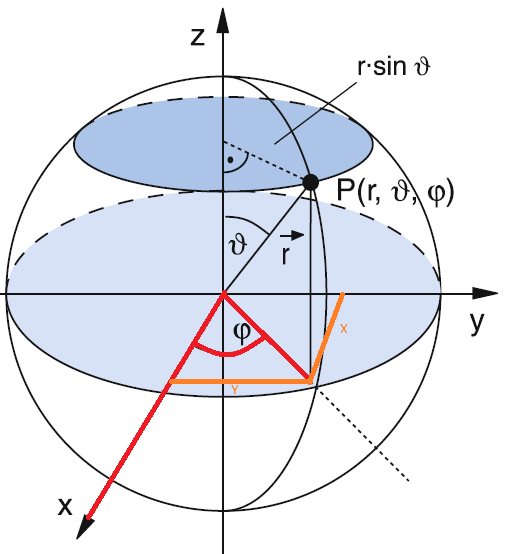
\includegraphics[width=0.5\linewidth]{images/02_methodology/spherical_coords.png}
    \caption[Spherical Coordinates adapted from \parencite{Demtröder2020-mw}.]{Spherical Coordinates in body frame adapted from \parencite{Demtröder2020-mw}. Shown in red is the angle between the projection of the vector $\vec{r}$ and the x-axis. Shown in orange are the~$x$ and~$y$ components used to calculate pitch and roll.}
    \label{fig:meth:spherical_coordinates}
\end{figure}

To rotate the body frame to the world frame, a rotation of~$\pi-\vartheta$ needs to be performed about the axis in the xy-plane perpendicular to the xy-projection of~$\vec{g}^{\mathrm{bf}}$, which is marked with the dotted line in fig.~\ref{fig:meth:spherical_coordinates}. This would align the gravity vector antiparallel to the z-axis in the world frame. This hypothetical axis is equivalent to the x-axis rotated by~$\varphi+\frac{\pi}{2}$ about the z-axis. A rotation of~$\varphi$ is performed about the z-axis to align the body frame's x-axis with the deflection of the gravity vector. The y-axis is in  a ninety degree angle to the x-axis, so we rotate about this as it does not matter if we had turned the x-axis by~$\varphi+\frac{\pi}{2}$ and rotated about this or if we rotate the x-axis by~$\varphi$ and then rotate about the y-axis, as they stand at a~90$^\circ$ angle to one another. After having performed the rotation of $\varphi$ about the z-axis, the second rotation of angle~$\vartheta$ about the y-axis aligns the z-axis antiparallel to the gravity vector. A rotation of~$-\varphi$ is then performed about the z-axis to restore the initial heading of the sensor. To determine what heading this is, the measured magnetometer vector is rotated to the world frame as described and is shown below.
\begin{equation}
    \vec{B}_{\mathrm{meas}}^{\ \mathrm{wf}}=R_z(-\varphi)R_y(\vartheta)R_z(\varphi)\vec{B}_{\mathrm{meas}}^{\ \mathrm{bf}}
\end{equation}
With the following rotational matrices:
\begin{align}
    R_z(\alpha)&=\begin{pmatrix}
                \cos\alpha & -\sin\alpha & 0 \\
                \sin\alpha & \cos\alpha & 0 \\
                0 & 0 & 1
                \end{pmatrix} \\
    R_y(\beta)&=\begin{pmatrix}
                \cos\beta & 0 & \sin\beta \\
                0 & 1 & 0 \\
                -\sin\beta & 0 & \cos\beta
                \end{pmatrix}
\end{align}

Seeing that Magnetic North is the direction in which the xy-projection of the magnetic field is pointing, the xy-projection of~$\vec{B}_{\mathrm{meas}}^{\ \mathrm{wf}}$ needs to be evaluated. The angle~$\psi\in[0,2\pi]$ is the angle between the x-axis of the world frame and the xy-projection of the magnetic field vector (in wf) minus the declination and equivalent to the gondola's heading. The declination~$\delta$ of the magnetic field describes the location dependant angle between True and Magnetic North.

By computing pitch, roll, and heading as described above, objectives 1 and 2 of this thesis are fulfilled.

Because we use numpy's atan2 function the -180\,$^\circ$ to 180\,$^\circ$ in mathematically positive sense have to mapped to the~0\,$^\circ$ to~360\,$^\circ$ of a compass in mathematically negative sense. 

\section{Reflection on Methodology \label{sec:meth:reflection_methodology}}